\chapter{ACCRETION DISKS}
    \label{chap:accretion_disks}
    \thispagestyle{empty}

    \mquote{not selected yet}{...}
    % TODO: citat!

    The term \emph{accretion} comes from a Latin word \emph{accrescere} which literarily means \emph{become larger}, and in astrophysics, we refer exactly to that process. That is the \emph{coming together and cohesion of matter under the influence of gravity to form larger bodies} (citace). One could easily argue that it is one of the most fundamental processes in the universe. From the giant galaxies to the tiniest rocks floating around in the solar system. All the stars, planets, and all there is were smashed together by gravity at some point in the past. Atom by atom, piece by piece, to form larger and larger structures. Even the dinosaurs probably met their fate by a city-sized asteroid that accreted Earth some 65 million years ago. 

\section{Accreting systems}
    Accretion is not only the mass moving and colliding but also energy taking different forms in the process. Depending on the nature of the accreting system and its central object, radiation of various types is emitted by the accreted matter as it loses energy. Under certain conditions, the matter flow forms an accretion disk often closely confined to the orbital plane. If we sort accreting astrophysical systems based on their size, radiation power, and a few other characteristics, we can devise a crude classification of them. We will briefly describe the accreting system types in the following sections. 

\subsection{Active galactic nuclei (AGN) and Quasar}
    The high-luminosity region containing a supermassive black hole in most galaxies' centers is refered to as \emph{Active Galactic Nucleus}. The radiative power of the AGN is usually higher than that of the whole host galaxy, and the radiation characteristics indicate that stars are not the primary source of this radiation. Instead, mass accretion onto the central supermassive black hole is the more likely source of this excess non-stellar power output. 

    The main distinguishing characteristic of AGNs is whether they are \emph{radio loud} or \emph{radio quiet}, which depends on the existence of jets that are the source of radio radiation. By \emph{jets}, we mean relatively narrow streams of accreted mass ejected from the black hole in both directions, roughly colinear with its axis of rotation. These mass ejections can travel at relativistic speeds. 
    
    Figure \ref{fig:centaurus_a_multiwave} shows the Centaurus A (NGC 5128) galaxy with a supermassive black hole in its center. This object is a typical \emph{radio loud} AGN. We can see both jets in the radio part of the spectrum and the accreted matter in other parts of the spectrum. For example, the galaxy's dust core is most apparent in visible light.

    \begin{figure}[t!]
        \centering
        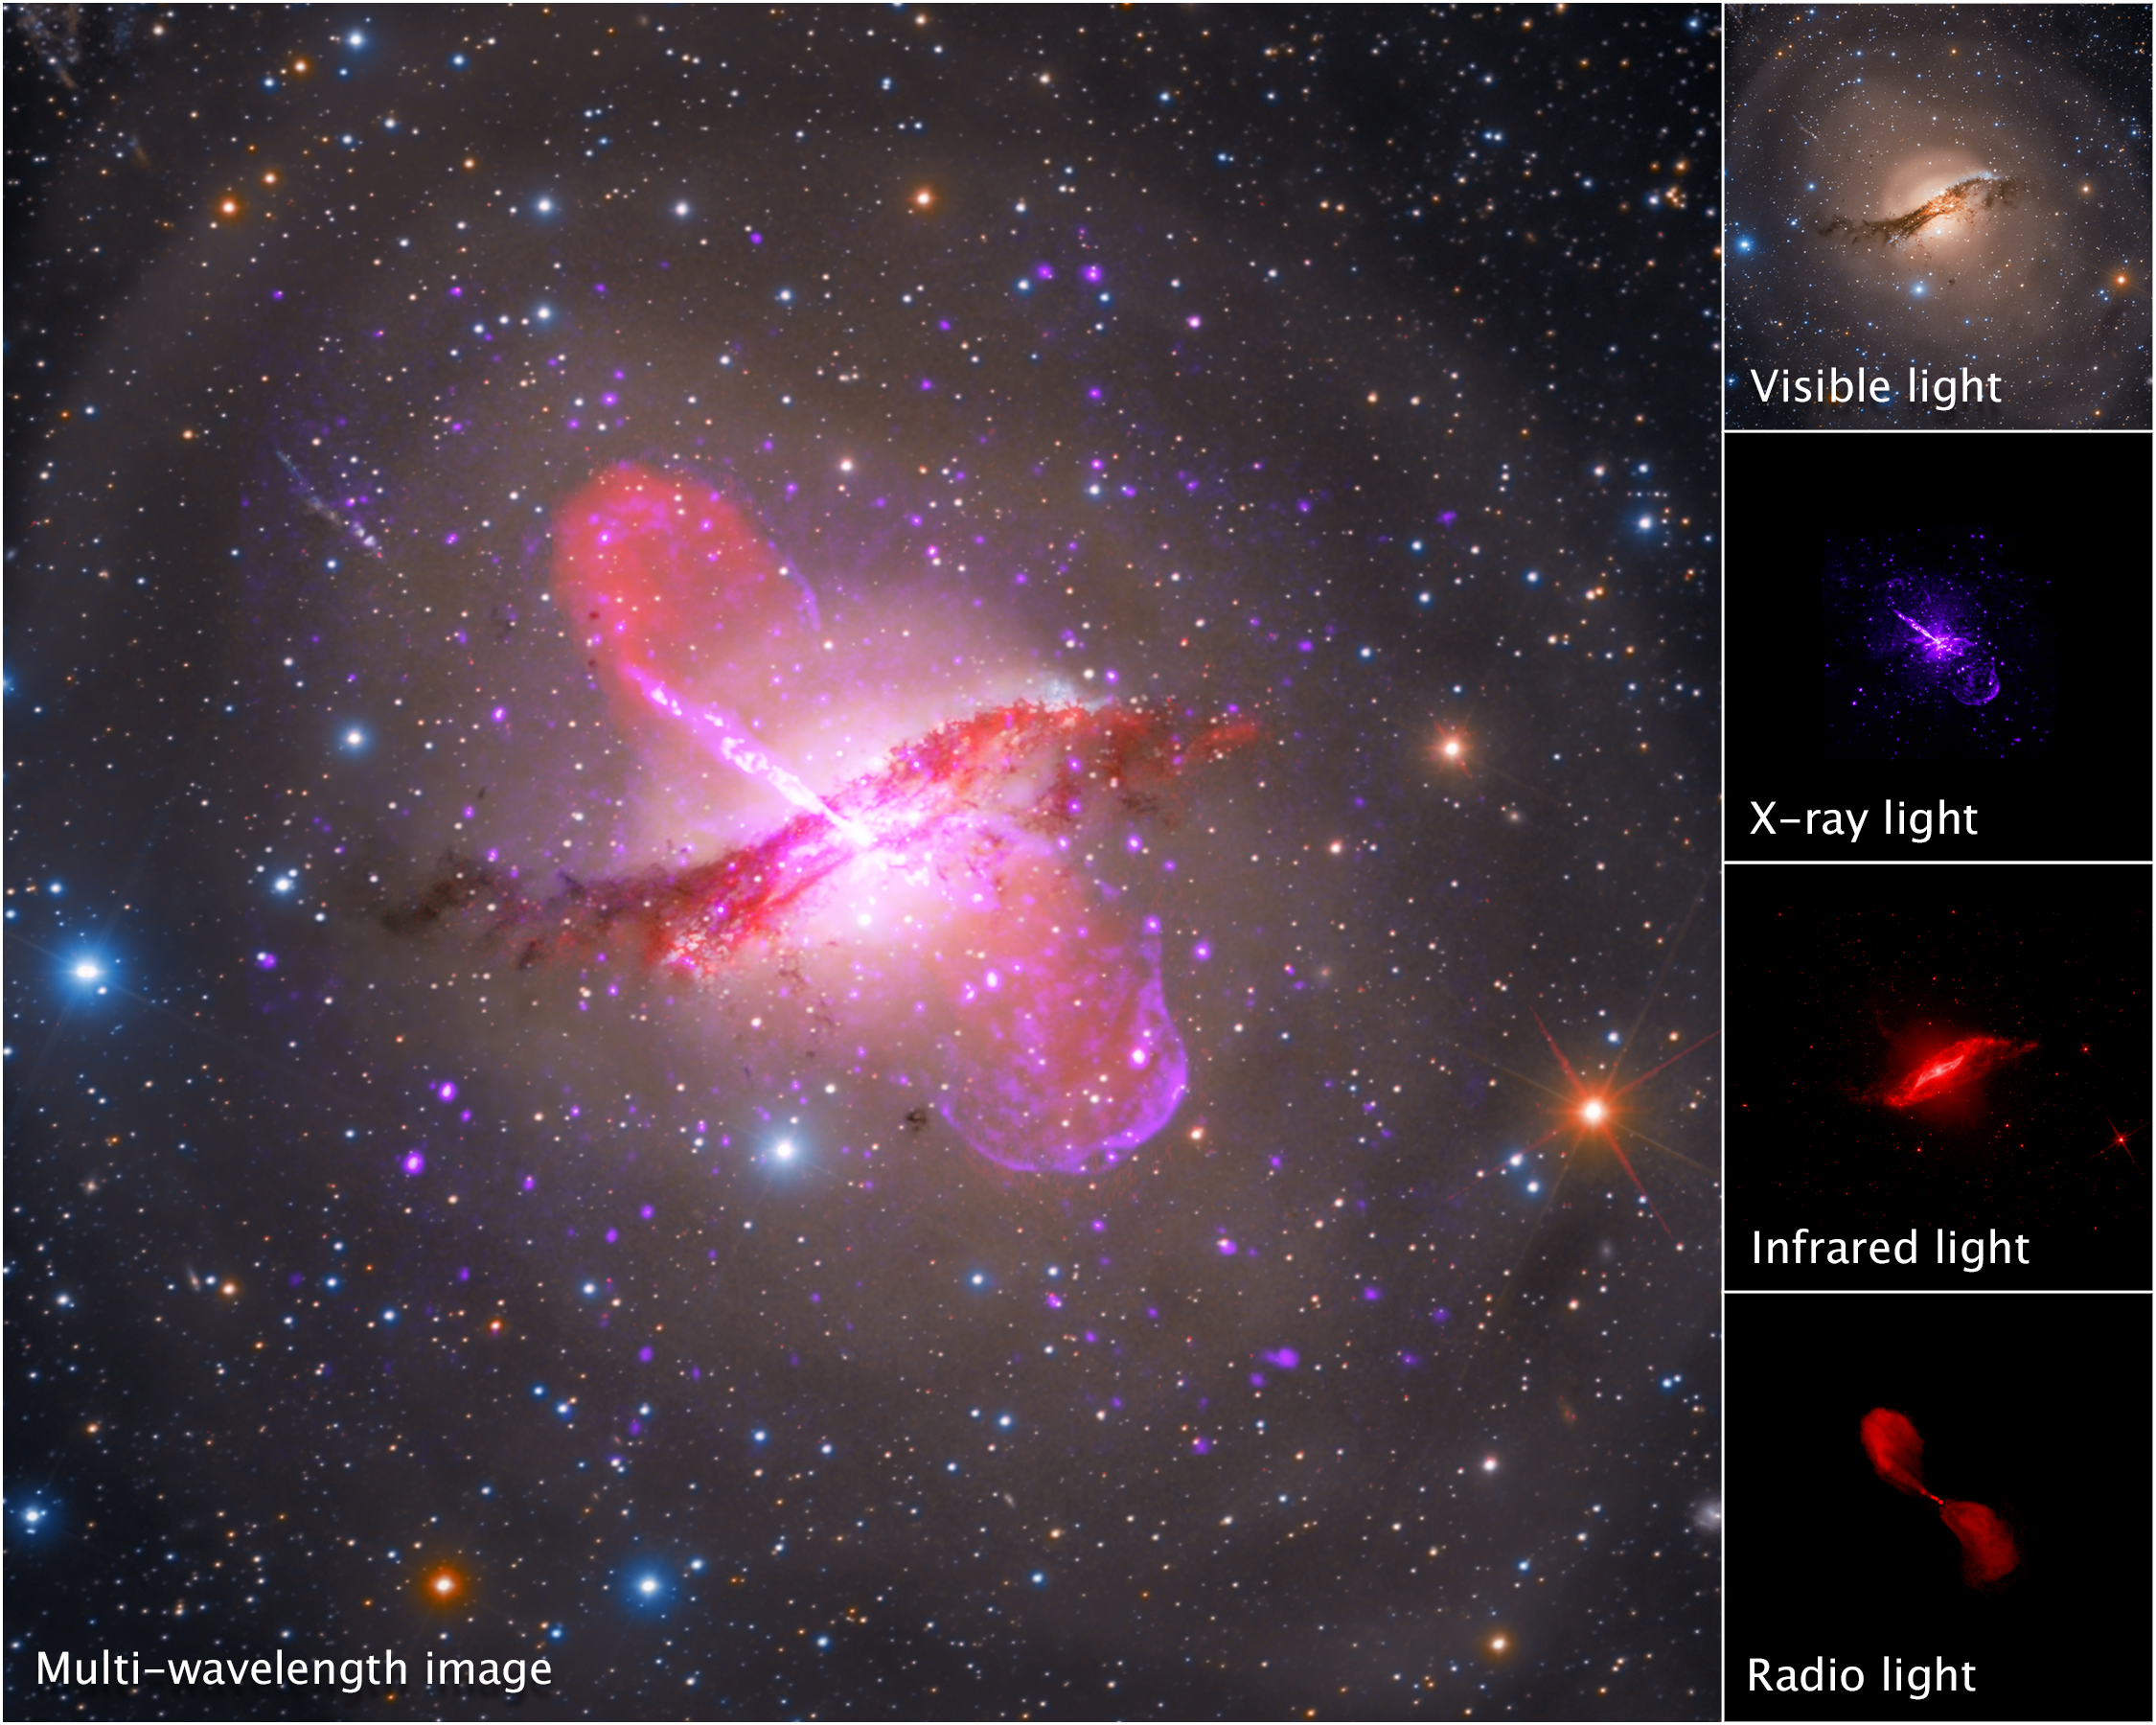
\includegraphics[width=\columnwidth]{img/multiwave_centaurus_a_agn.png}
        \caption{Multi-wavelength composition (left) and multiple narrow wavelength observations (right) of Centaurus A. Taken from \citep{nasa_img_centaurus_a}}
        \label{fig:centaurus_a_multiwave}
    \end{figure}

    A particular sub-category of AGN is Quasars. The name \emph{Quasar} is a contraction of the phrase \emph{quasi-stellar radio source} because, in the 1950s, they were detected as radio sources of unknown physical characteristics and also in visible light as faint \emph{star-like} sources. However, they are nothing like stars. These highly luminous objects are observed to the highest values of redshift. The current record holder for the most distant Quasar is the J0313-1806 detected at redshift $z = 7.64$ by \citep{wang2021}. 

    Due to the extreme distance, it is impossible, at least with today's methods, to distinguish the active core (i.e., the supermassive black hole), whose mass can range from $10^6 M_{\odot}$ to $10^{9} M_{\odot}$. To this day, more than a million quasars have been discovered, with the closest known Markarian 231 (UGC 8058) at 581 million light-years away \citep{gaia2018}. 


\subsection{X-ray binaries (XB)}
    The main sequence star in orbit around a neutron star (NSB - \emph{Neutron Star Binary}) or a black hole (BHB - \emph{Black Hole Binary}) is referred to as a \emph{X-ray binary} (XRB). The gravitational potential of these systems is strong enough that the accreted matter produces energy output up to the X-rays. Based on the mass of the primary component (i.e., the accretor), this class of binary stars is also usually split between \emph{Low-mass X-ray binary} (LXRB) and \emph{High-mass X-ray binary} (HXRB). 

    Most XRB objects go through periods of high activity when they emit twin jets at relativistic speed, not that dissimilar to AGN but at a smaller scale, and then a period of relative quiescence.

    In the special case, when the accretor is the strongly magnetized young neutron star, the accretion disk is truncated by its magnetic field or not present at all, and the matter transfers onto the neutron star by \emph{column accretion}.
    
    %% TODO: Muj Cygnus X-1 pro demonstraci

\subsection{Young stellar objects (YSO)}
    When a proto-star is formed from a collapsing molecular cloud, the gas and solid particles envelope forms a rotating protoplanetary accretion disk. Instabilities and self-gravity in the disk's body eventually lead to planets and other smaller objects forming. The proto-star is only detectable in infrared due to the relatively dense surrounding matter that obscures it. 

    The YSO classification consists of five classes (0-IV) based on the infrared and visible spectral energy distribution. Class 0 is a collapsing molecular cloud. Classes I to III are YSO with a formed proto-planetary disk in various stages of evolution, and lastly, class IV refers to a fully formed zero-aged star. 

    \begin{figure}[h]
        \centering
        \includegraphics[width=\columnwidth]{img/jwst_protostar_l1527.png}
        \caption{Proto-star L1527 captured by Near-Infrared-Camera (NIRCam) onboard the JWST. Taken from \citep{nasa_img_l1527}}
        \label{fig:jwst_protostar_l1527}
    \end{figure}


    As a side note, the \emph{James Webb Space Telescope} (JWST) was released only a year ago, on December 25, 2021. It is equipped with multiple near-infrared and infrared instruments, so it is literarily able to see through the clouds of such objects and uncover the stars being born. Due to JWST's observational capabilities and the sheer size of its primary mirror, we have something to look for in this particular field of astrophysical research. The first glimpses of JWST observations demonstrate the spectacular Figure \ref{fig:jwst_protostar_l1527}, showing the proto-star L1527 captured by the Near-Infrared-Camera (NIRCam). 

\subsection{Gamma-ray bursts (GRB)}
    Highly energetic, collimated flashes of $\gamma$-rays that can last tens of milliseconds up to several hours are called \emph{Gamme-ray burts} (GRB). These are considered the most energetic events in the observable universe. In addition, GRBs are accompanied by simultaneous radiation on longer wavelengths (e.g., X-ray) and a follow-up slowly fading afterglow that may be observable for up to several years. 

    It is theorized that the possible origin of GRBs may be a compact object merger or a \emph{collapsar} (i.e., the failed supernovae). The observations indicate the formation of a black hole with an accretion disk surrounding it and a high mass accretion rate \citep{piran2005}.

    One of the brightest detected GRB 221009A (Swift J1913.1+1946) was detected very recently on October 9, 2022, by the orbital \emph{Neil Gehrels Swift Observatory} \citep{grb_221009a}. It is also one of the closest observed GRBs. 

    %% TODO: obrazek GRBu??? -> spis neni potreba

\subsection{Cataclysmic variables (CV)}
    We are particularly interested in CVs in this study because our modeling efforts in the latter chapters focus on generic CV systems. Unlike the LMXB or HMXB, where the primary component is either a black hole or neutron star, the accretor in CV is a White Dwarf (WD), and its companion is a late-type star. Due to its nature, this system has a relatively weaker gravitational potential; therefore, its radiation energy output is lower than that of the XRB and is comparable in size to planetary or Earth-Moon-like systems. 

    The primary WD is a stellar core remnant composed of very dense electron-degenerate gas, and its size can be approximated by the \emph{mass-radius ratio} \citep{shapiro1983}

    \begin{equation}
        r_{\textrm{in}} \sim M^{-1/3}_{\textrm{p}},
        \label{eq:mass_radius_ratio}
    \end{equation}

    where $M_{\textrm{p}}$ represents the WD's mass and $r_{in}$ its radius, which also corresponds to the inner boundary layer radius of the accretion disk.

    The secondary component star fills its Roche lobe, and the overflowing matter falls onto the WD through the Langrangian point $L_1$ \citep{warner1995}. If the WD is not magnetized or weakly magnetized, the gas stream forms an accretion disk around the WD that eventually reaches its surface. In the case of strongly magnetized WD, the accretion disk is truncated or non-existent, and the magnetic field lines direct the accretion flow (citace). 

    Another important parameter of the CV binary system is its component separation distance, closely related to individual component masses. It determines the accretion disk size because the gravitational potential constrains its outer edge. The outer disk radius is calculated

    %% TODO: Citace vypoctu? Podrobnejsi vyjadreni

    \begin{equation}
        r_{out} = d \left[ \frac{M_{\textrm{s}}}{3(M_{\textrm{p}}+M_{\textrm{s}})} \right]^{1/3},
        \label{eq:disk_outher_radius}
    \end{equation}

    where $M_{\textrm{s}}$ represents the secondary component's mass and $d$ is the distance between the components. Equations \eqref{eq:mass_radius_ratio} and \eqref{eq:disk_outher_radius} give us the inner and outer constraints to define the geometry of the model, which we will define in the latter chapters of this study.   

\section{Accretion disks models}
    For the accreting matter that dissipates energy and is not supported by internal pressure, the matter will form an accretion disk, which is its minimal energy configuration. The falling matter must lose angular momentum to reach the central object. This process is done through a \emph{viscous disipation} that is key in transporting the angular momentum outward and heats the disk. The nature and magnitude of the viscous processes are the questions of accretion disk modeling because they are the critical factor determining the disk size, shape, optical dept, and radiation properties. It still needs to be better understood in the case of accretion disk matter flow because the disk's body consists of a sheering, radiative, and supersonic medium with a high Reynold's number \citep{pringle1981}, and that is quite a challenging problem to model. 

    Then there is a question of magnetic fields. The central object (i.e., WD or NS) may or may not be magnetized. Some objects rotate very fast. For example, NS rotation periods range from a couple of milliseconds to tens of seconds. The temperature and composition of the material inflow can widely differ depending on the characteristics of the secondary object. All those factors add up and create a complex non-linear accretion environment. Therefore, when modeling such a complex and dynamic astrophysical system, we are inevitably forced to make some simplifications, neglections, and approximations. 

    In many cases, the accretion disk is closely confined to an orbital plane, so in the first approximation, we may regard the disk's matter flow as two-dimensional, ad we call this the \emph{thin disc approximation}. This simple yet very effective simplification enables the creation of a very elaborate accretion model's theory, but with reduced complexity, \citep{acpow}.

\subsection{Sub-Eddington accretion disks}
    The standard vertically \emph{thin} accretion disk is formed under the conditions of sub-Eddington accretion rate and very high opacity. The Eddington limit
    
    \begin{equation}
        L_{\mathrm{E}} = 1.38 \cdot 10^{38} (M / M_{\odot}) 
    \end{equation}

    is the maximum luminosity of a radiating body in hydrostatic equilibrium, which means the radiation and gravitational forces acting in opposite directions are in balance. The accreting matter follows very tight spiraling orbits that are almost Keplerian. Moreover, thin disks have a relatively high luminosity with spectral energy distribution closely resembling a \emph{black body} radiation. Thin disks theory was devised almost independently by \citep{lyndenbell1974}, \citep{pringle1981}. Under the umbrella of \emph{standard thin disks} is also the Shakura-Sunyaev $\alpha$-disc model, which is described more closely in Section \ref{sec:alpha_model_definition}. This model is particularly interesting to us because part of our simulation efforts in the latter chapters is focused on the $\alpha$ parameter modeling.

    In the case of the central object in the thin disc system being a black hole, the models need to deal with relativistic effects in its proximity. Researchers D. N. Page and K. S. Thorne provided such a theory in \citep{page1974}, which was later used by \citep{luminet1979} and \citep{marck1996} to generate synthetic images of Keplerian disk around a black hole distorted by intense gravitational lensing. Figure \ref{fig:bh_warped} shows a more recent simulation example of such a synthetic image. 

    \begin{figure}[h]
        \centering
        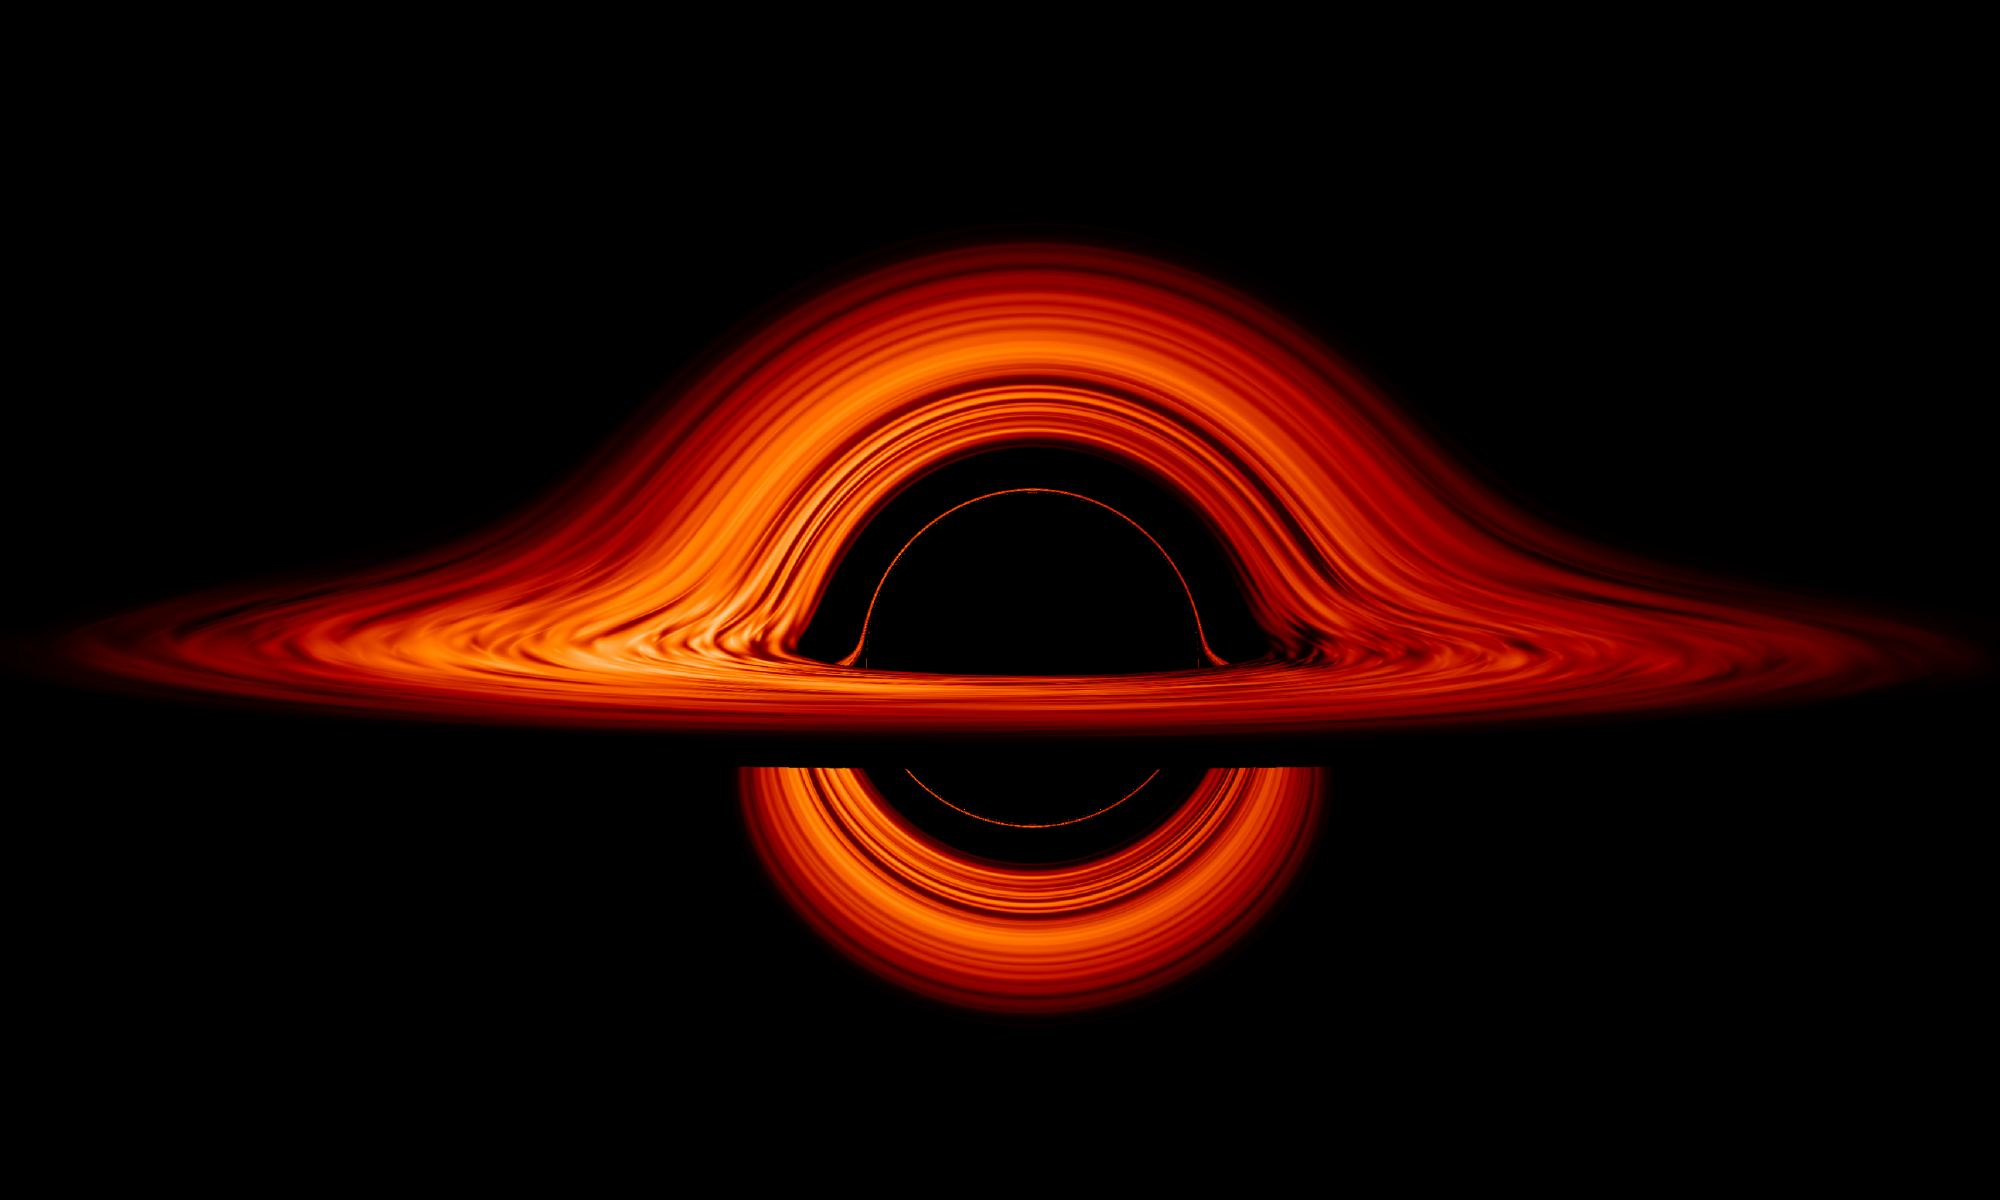
\includegraphics[width=1.0\columnwidth]{img/bh_warped.jpg}
        \caption{Visualization of a black hole accretion disk. The observer's image is warped by extreme gravitational lensing and highly depends on the observer's inclination. Taken from \citep{nasa_img_bh_warped}}
        \label{fig:bh_warped}
    \end{figure}

    As a side note, these simulated images found their way even to a broader audience through pop-cultural references. Professor Thorne himself worked as a science advisor for Christopher Nolan's 2014 movie Interstellar, in which very accurate VFX renders of a supermassive black hole with an accretion disk were used. 

    The other type of sub-Eddington disk that, forms when the opacity is very low, is called ADAF (\emph{Advection-Dominated Accretion Flows}), and it was predicted by \citep{ichimaru1977}. ADAFs are radiatively very inefficient, because the cooling is done dominantly by advection (i.e., heat capture in the matter) and not by radiation. Therefore they are very hot, geometrically extended and more similar in shape tho a sphere than a flat disk \citep{acpow}.

\subsection{Super-Eddington accretion disks}
    Observations of higly luminous quasars at high values of redshift ($z \sim 7$), like the afformetioned J0313-1806, suggests that in order to grow s supermassive black hole with mass $M_{\mathrm{BH} > 10^9 M_{\odot}}$ in under a billion years after the big-bang the accretion rate of such object needs to break the Eddington limit. However, it is theorized that the Eddington limit could be breaked by non-spherical geometry and instabilities \citep{brightman2019}.

    As our technological capabilities progress and enables observations of these extremly distand and old objects, the details of super-Edington accretion mechanism remain uncler. This topic is important for understanding the processes behing the growt of first supermassive black holes and teir impact on their host galaxies.

\subsection[Shakura-Sunyaev $\alpha$-Disc model]{Shakura-Sunyaev $\alpha$-disc}
    \label{sec:alpha_model_definition}
    In 1973, N. I. Shakura and R. Sunyaev proposed an accretion disk model whose source of increased viscosity are the turbulent flow patterns in the disk's body \citep{shakura1973}. This model applies if the modeled system is a \emph{thin disk}, and because of that, it is considered that all material in the disk's body is near its surface, allowing the thermal emission to escape freely. Therefore, self-absorption processes are insignificant. 

    Utilizing equations of hydrostatic equilibrium and Kramer's opacity law on the two-dimensional disk, we can devise a set of equations that describe the local disk structure \citep{acpow}

    \begin{align}
    \begin{split}
        \rho &= \Sigma / H, \\
        H &= c_{\mathrm{s}} R^{3/2} / (GM)^{1/2}, \\
        c_{\mathrm{s}}^2 &= P / \rho, \\
        P &= \frac{\rho k T_{\mathrm{c}}}{\mu m_p} + \frac{4 \sigma}{3 c}T_c^4, \\
        \frac{a \sigma T_{\mathrm{c}}^4}{3 \tau} &= \frac{3GM\dot{M}}{8 \pi R^3}, \\
        \tau &= \Sigma \kappa_{\mathrm{R}}(\rho, T_{\mathrm{c}}) = \tau(\Sigma, \rho, T_{\mathrm{c}}), \\
        \nu \Sigma &= \frac{\dot{M}}{3 \pi} \left[ 1 - \left( \frac{R_*}{R} \right)^{1/2} \right], \\
        \nu &= \nu(\rho, T_{\mathrm{c}}, \Sigma, \alpha, ...).
    \end{split}
    \label{eq:alpha_model_prescription}
    \end{align}

    The set of equations \eqref{eq:alpha_model_prescription} contains eight unknowns: density $\rho$ and temperature $T_{\mathrm{c}}$ of disk's mid-plane, scale height $H$ of the disk, the speed of sound in the medium $c_s$, the sum of gas and radiation pressure $P$, area density $\Sigma$, optical depth $\tau$, and viscosity $\nu$. These unknowns are solved as functions of: accretion rate $\dot{M}$, the central object's mass $M$, the radius of a specific point in the disk $R$, and free parameter $\alpha$. Moreover, $R_*$ represents the radius where angular momentum stops being transported outwards. Assuming that the values $\rho$ and $T_{\mathrm{c}}$ enable the approximation of Rosseland mean opacity using Kramer's law

    \begin{equation}
        \kappa_{\mathrm{R}} = 5 \cdot 10^{24} \rho T_{\mathrm{c}}^{-7/2} \si{\cm^2 \gram^{-1}},
    \end{equation}


    the viscosity of the disk's medium is estimated

    \begin{equation}
        \nu = \alpha c_{\mathrm{s}} H,
    \end{equation}

    where $c_{\mathrm{s}}$ represents the speed of sound in the medium. $H$ represents the scale height of the disk limiting the subsonic turbulent eddies size. The free parameter $\alpha$ ranges between zero (no accretion) and approximately one. Solving the equations \eqref{eq:alpha_model_prescription} with the assumption $\mu = 0.615$ (fully ionized gases), we get a set of relations representing the Shakura-Sunyaev $\alpha$-disc solution \citep{acpow}  

    \begin{align}
    \begin{split}
    \Sigma &= 5.2 \alpha^{-4/5} \dot{M}^{7/10}_{16} m^{1/4}_1 R^{-3/4}_{10} f^{14/5}\ \mathrm{g\ cm^{-2}}, \\
    H &= 1.7 \times 10^8 \alpha^{-1/10} \dot{M}^{3/20}_{16} m^{-3/8}_1 R^{9/8}_{10} f^{3/5}\ \mathrm{cm}, \\
    \rho &= 3.1 \times 10^{-8} \alpha^{-7/10} \dot{M}^{11/20}_{16} m^{5/8}_1 R^{-15/8}_{10} f^{11/5}\ \mathrm{g\ cm^{-3}}, \\
    T_{\mathrm{c}} &= 1.4 \times 10^4 \alpha^{-1/5} \dot{M}^{3/10}_{16} m^{1/4}_1 R^{-3/4}_{10} f^{6/5}\ \mathrm{K}, \\
    \tau &= 190 \alpha^{-4/5} \dot{M}^{1/5}_{16} f^{4/5}, \\
    \nu	&= 1.8 \times 10^{14} \alpha^{4/5} \dot{M}^{3/10}_{16} m^{3/4}_1 R^{3/4}_{10} f^{6/5}\ \mathrm{cm^2\ s^{-1}},  \\
    v_{\mathrm{R}}	&= 2.7 \times 10^{14} \alpha^{4/5} \dot{M}^{3/10}_{16} m^{-1/4}_1 R^{-1/4}_{10} f^{-14/15}\ \mathrm{cm\ s^{-1}},  \\
    \mathrm{with}\ f &= \left[ 1 - \left( \frac{R_*}{R} \right)^{1/2} \right]^{1/4}, \\
    \end{split}
    \label{eq:alpha_model_solution}
    \end{align}

    where $f$ represents the boundary layer function. $\dot{M}_{16}$, $R_{10}$, and $m_1$ are transformed to be represented in typical sizes of disk quantities

    \begin{align}
    \begin{split}
        \dot{M}_{16} &= \dot{M} / 10^{16} \si{\gram \second^{-1}}, \\
        R_{10} &= R / (10^{10} \si{cm}), \\
        m_1 &= M / M_{\odot}.
    \end{split} 
    \end{align}

    Figure \ref{fig:plot_alpha_H_T} shows $T_{\mathrm{c}}$ and $H$ solution examples using different values of free parameter $\alpha$ for the same accretion disk system.

    \begin{figure}[H]
        \centering
        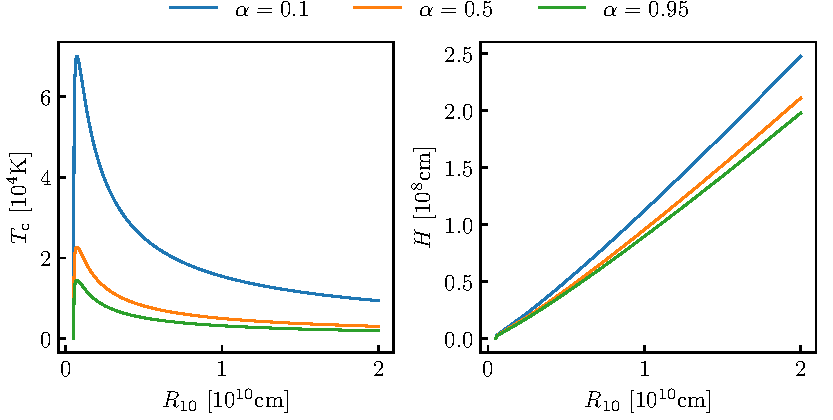
\includegraphics[scale=1.0]{img/plot_alpha_H_T.pdf}
        \caption{$\alpha$-disk model solution examples. Chosen central object's mass is $m_1 = 0.8$. Mid-plane temperatue $T_{\mathrm{c}}$ solution (left) and scale height $H$ (right).}
        \label{fig:plot_alpha_H_T}
    \end{figure}
